\documentclass{acm_proc_article-sp}
\usepackage{amsmath}
\usepackage{hyperref}
\usepackage{listings}

\lstset{
  language=Lisp,
  %labelstep=5,
  frame=trbl,
  %indent=15pt,
  %indent=0pt,
%  xleftmargin=-10pt,
%  xrightmargin=10pt,
  showlines=false,
  basicstyle=\small\tt,
  stringstyle=\itshape,
  showstringspaces=false%,
}

\begin{document}

\conferenceinfo{6.945}{2008 Cambridge, MA USA}

\title{BioHacker}

\numberofauthors{3}

\author{
\alignauthor
Nada Amin\\
       \affaddr{MIT}\\
       \email{namin@mit.edu}
\alignauthor
Dan Wheeler\\
       \affaddr{MIT}\\
       \email{lowe@mit.edu}
\alignauthor
Jeremy Zucker\\
       \affaddr{MIT}\\
       \email{zucker@broad.mit.edu}
}

\date{May 14, 2008}

\maketitle

%\begin{abstract}
%\input{abstract}
%\end{abstract}

%\category{}{}{}

%\terms{}
%\keywords{}

% to get word count:
% ps2ascii file.pdf | wc -w

%\begin{description}
%\item[Abstract Reference Number] 0509
%\item[Word Count] 495
%\end{description}

\section{Introduction}
Despite a plethora of sequenced genomes, a paucity of genome-scale
metabolic models have been published thus far.  The bottleneck comes
from the extensive manual effort is currently required to reconstruct
the metabolic network.  In order to be effective, a model of
metabolism should be {\em coherent}, in the sense that the model
should obey physico-chemical constraints, such as charge and mass
balance.  It should be {\em complete}, in the sense that all genes
that code for metabolic enzymes should be part of the model.
Finally, the model should be {\em consistent} with conditional gene
essentiality experiments that measure growth/no-growth under various
different nutrient media and gene knockouts.

Inspired by computer models of skill acquisition\cite{HACKER} and
robot scientists that automate the scientific process\cite{king2004},
we have developed {\tt BIOHACKER} as a network debugging tool to
detect incoherence in the network, generate reasonable hypotheses for
filling in gaps in incomplete networks, and predict sufficient
nutrient sets that are consistent with conditional essentiality
experiments.



\section{Network Debugger}
\subsection{Overview}

The user of the network debugger provides a model of the network and a
set of experiments. For each experiment, the network debugger assesses
whether the experiment is consistent with the model, explaining why
(with a queryable proof) or why not (with queryable minimal fixes).

\subsection{Demonstration}

For purpose of demonstration, we will use the small network shown in Figure~\ref{figure:network}.
The user code which specifies this network model is shown in Listing~\ref{listing:network-model-def}.

The set of experiments in Listing~\ref{listing:experiments} tests our
model. In order to test our system, we purposefully introduced some
inconsistencies in our model with respect to the experiments:
\begin{itemize}
\item {\small\tt reaction r1} has its reactants and products swapped.
\item {\small\tt reaction r2} has no enzymes catalyzing it.
\item {\small\tt reaction r4} shouldn't actually be part of our model.
\end{itemize}

\begin{figure}[htb]
\centering
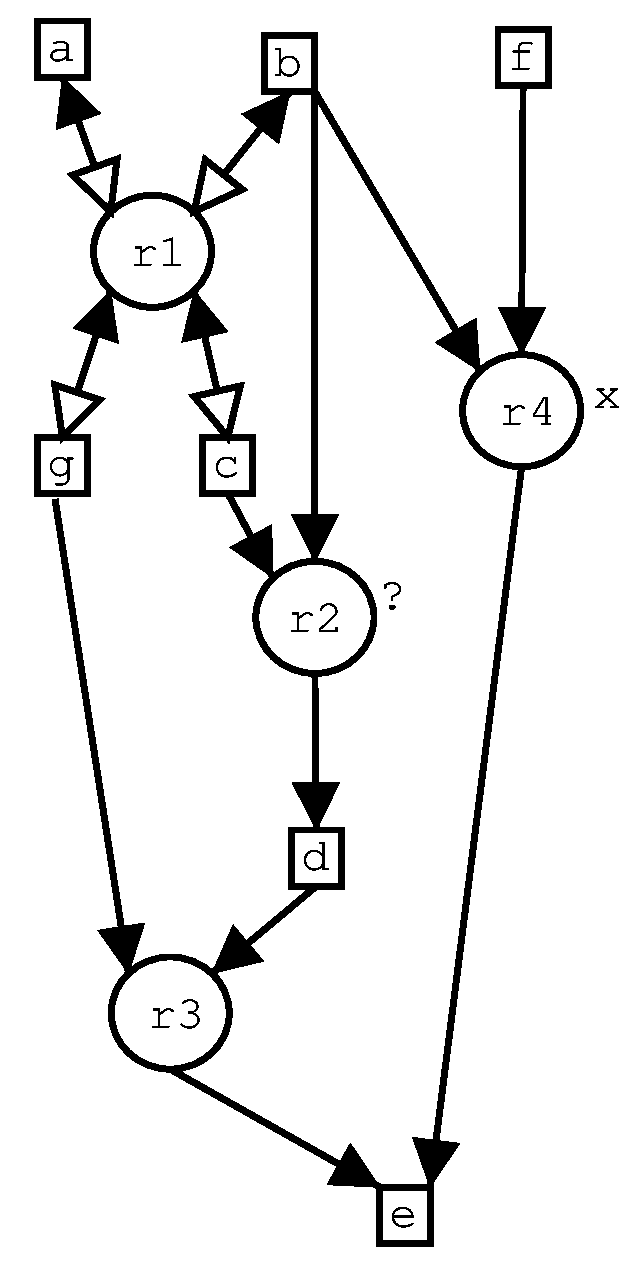
\epsfig{file=demo.eps, height=3in, width=1.5in}
\caption{\label{figure:network} Example Metabolic Network}
\end{figure}

\begin{lstlisting}[label={listing:network-model-def},caption={Network Model}]
(network-debugger demo 
  :debugging t 
  :abducting t 
  :rules :extended-reactions)

(reaction r1 
  :reactants (c g) 
  :products (a b) 
  :enzymes (e1))

(reaction r2 
  :reactants (b c) 
  :products (d))

(reaction r3 
  :reactants (d g) 
  :products (e) 
  :enzymes (e3))

(reaction r4 
  :reactants (b f) 
  :products (e) 
  :enzymes (e4))

(enzyme e1 g1)
(enzyme e3 g3 g3p)
(enzyme e4 g4)
\end{lstlisting}

\begin{lstlisting}[label={listing:experiments},caption={Experiments}]
(experiment 
 positive 
 (a b d) 
 :growth? t 
 :essential-compounds (a e))

(experiment 
 negative 
 (a) 
 :growth? nil 
 :essential-compounds (a e))

(experiment 
 false-positive 
 (a b f) 
 :growth? nil 
 :essential-compounds (a e) 
 :knock-outs (g1))

(experiment
 false-negative
 (a b)
 :growth? t
 :essential-compounds (a e))
\end{lstlisting}

We immediately get the following feedback when loading the set of
experiments:
\begin{itemize}
\item Experiments {\small\tt positive} and {\small\tt negative} are consistent with the model.
\item Experiment {\small\tt false-positive} is not consistent with the model. Needs:
\begin{itemize}
\item {\small\tt ( (NOT (GENE-ON G4)) )}
\end{itemize}
\item Experiment {\small\tt false-negative} is not consistent with the model. Needs:
\begin{itemize}
\item {\small\tt ( (NUTRIENT E) )}
\item {\small\tt ( (NUTRIENT D) )}
\item {\small\tt ( (REACTION-ENABLED R2) )}
\item {\small\tt ( (NUTRIENT F) )}
\end{itemize}
\end{itemize}

Notice that the network debugger suggested enabling {\small\tt
reaction r2} and disabling {\small\tt reaction r4} to fix our model.

Once an experiment is consistent with the model, the network debugger
can explain why by providing a proof and allowing the user to query
this proof. For example, after loading the experiment {\small\tt
positive}, the user can type {\small\tt (explain
'experiment-consistent)} to get a Suppes-style proof. The user can
query the facts that play a role in the proof using {\small\tt
all-antecedents}. For example, {\small\tt (all-antecedents
'experiment-consistent '((reaction-enabled ?r) (reaction-reversible
?r)))} returns {\small\tt ((REACTION-ENABLED R3) (REACTION-ENABLED R1)
(REACTION-REVERSIBLE R1))}. As a shortcut, it is possible to list
reactions that had to explicitly be assumed reversible for the proof:
{\small\tt (explicit-reversibility)} returns {\small\tt
(R1)}. Similarly, {\small\tt (explicit-gene-expression)} returns which
genes had to explicitly be assumed on for the proof.

\subsection{Specification}
\subsection{Implementation}

\section{Results} 
To test the ability of the {\tt NETWORK DEBUGGER} to debug real data, we
exported the EcoCyc\cite{ecocyc}\cite{romero2001} representation of the {\em E. coli}
metabolic network into the {\tt NETWORK DEBUGGER} domain data format, generating
929 {\tt reaction}s, 836 {\tt enzyme}s, and 251 {\tt pathway} premises.

To ensure that our model would grow on at least one nutrient media, we generated an {\em in silico} rich medium
set by taking the union of all proper reactants of each pathway in the model, as shown in Listing~\ref{listing:richMedia}

\begin{lstlisting}[label={listing:richMedia},caption={{\em E. coli} rich media}]
(defun make-rich-media (pwy-list filter-p)
  `(experiment 
    growth 
    (nutrients 
     ,@(remove-duplicates 
	(loop for pwy in pwy-list
	   when (funcall filter-p pwy)
	   append (multiple-value-bind
			(all-reactants 
			 proper-reactants 
			 all-products 
			 proper-products)
		      (substrates-of-pathway pwy)
		    proper-reactants)))) (OFF)))
\end{lstlisting}

We then selected as our essential compounds the full set of amino acids, nucleic acids, cytoplasmic membrane components,
outer membrane components, and cell wall components as shown in Listing~\ref{listing:essentialCompounds}

\begin{lstlisting}[label={listing:essentialCompounds},caption={{\em E. coli} essential compounds}]
(setq *amino-acids*
  '(L-ALPHA-ALANINE ARG ASN L-ASPARTATE CYS GLN 
    GLT GLY HIS ILE LEU LYS MET PHE PRO SER THR 
    TRP TYR VAL))

(setq *dna-and-rna*
  '(DATP TTP DGTP DCTP ATP UTP GTP CTP))

(setq *cytoplasmic-membrane*
  '(L-1-PHOSPHATIDYL-ETHANOLAMINE CARDIOLIPIN 
    L-1-PHOSPHATIDYL-GLYCEROL))

(setq *outer-membrane* '(C6))
(setq *cell-wall*
  '(BISOHMYR-GLC ADP-L-GLYCERO-D-MANNO-HEPTOSE 
    KDO UDP-GLUCOSE UDP-GALACTOSE DTDP-RHAMNOSE 
    GDP-MANNOSE N-ACETYL-D-GLUCOSAMINE))
\end{lstlisting}

Surprisingly, even with this rich media, we were still unable to produce compound {\tt C6} (lipid intermediate II)

By manual checking, we discovered that the reason for this is that an upstream reaction, {\tt UDPNACETYLMURAMATEDEHYDROG-RXN }, in the Peptidoglycan biosynthesis pathway was reversed, making the entire chain of downstream metabolites unproduceable. 

Once this bug was discovered,  we added a new rule to our set of strategies so that
 if a metabolite is unproducable, the system tries to reverse
reactions with unknown reversibilities to see if that will
solve the problem.  

Interestingly, it has been shown that for many metabolic reconstructions,
that ''the dominant flow restoration mechanism is directionality
reversals of existing reactions in the respective
models''\cite{kumar2007}

Once we debugged this problem, we wished to reduce the rich medium to a nutrient set that was still
capable of producing growth. By querying the {\tt explain} mechanism of the underlying TMS, we were able to make the following
sufficient nutrient set prediciton as shown in Listing~\ref{listing:sufficientNutrientSet}.
\begin{lstlisting}[label={listing:sufficientNutrientSet},caption={{\em E. coli} predicted sufficient nutrient set}]
(GLN ASN THR LEU VAL ILE TRP PHE TYR CYS MET 
     LYS GLY ARG HIS PRO UDP-GALACTOSE 
     UDP-GLUCOSE RIBULOSE-5P 
     ADP-L-GLYCERO-D-MANNO-HEPTOSE GLC-1-P 
     TTP FRUCTOSE-6P 3-OHMYRISTOYL-ACP GLT 
     NADPH PHOSPHO-ENOL-PYRUVATE 
     MESO-DIAMINOPIMELATE L-ALPHA-ALANINE 
     D-ALANINE UDP-N-ACETYL-D-GLUCOSAMINE 
     UNDECAPRENYL-P GTP GLYCEROL-3P SER
     CDPDIACYLGLYCEROL METHYLENE-THF UTP 
     CTP UDP |Red-Glutaredoxins|
     |Red-Thioredoxin| |Reduced-flavodoxins| 
     CDP ATP WATER
     DIACETYLCHITOBIOSE-6-PHOSPHATE)
\end{lstlisting}
This sufficient nutrient set allowed us to focus on reactions and pathways that could produce these compounds starting
with experimentally determined nutrient sets, such as Middlebrook growth medium L9, as described in \cite{joyce2006}.


Finally, we then converted 13750 conditional gene essentiality experiments performed by
Covert et al\cite{covert2004} and for each condition, we recorded
whether the {\em E. coli} model's predictions of growth were
consistent or inconsistent with the experimental results. as shown in Listing~\ref{listing:biolog-experiments}.

\begin{lstlisting}[label={listing:biolog-experiments},caption={{\em E. coli} conditional essentiality experiments}]
(experiment in_vivo_EG11074_ala-D_nh4 
	    ( CARBON-DIOXIDE PROTON WATER 
			     AMMONIUM 
			     SULFATE 
			     D-ALANINE |Pi| 
			     OXYGEN-MOLECULE )
   :growth?  T
   :essential-compounds 
   ( L-ALPHA-ALANINE ARG ASN L-ASPARTATE CYS
     GLN GLT GLY HIS ILE LEU LYS MET PHE PRO 
     SER THR TRP TYR VAL DATP TTP DGTP DCTP 
     ATP UTP GTP CTP 
     L-1-PHOSPHATIDYL-ETHANOLAMINE CARDIOLIPIN
     L-1-PHOSPHATIDYL-GLYCEROL C6 BISOHMYR-GLC
     ADP-L-GLYCERO-D-MANNO-HEPTOSE KDO 
     UDP-GLUCOSE  UDP-GALACTOSE DTDP-RHAMNOSE 
     GDP-MANNOSE N-ACETYL-D-GLUCOSAMINE )

   :knock-outs ( EG11074 )
   :knock-ins Nil
   :toxins Nil
   :bootstrap-compounds Nil)

\end{lstlisting}

We found that most of the model predictions were false negatives
due to the existence of uninstantiated generic reactions. Inspired by
the symbolic computational approach to infer novel biochemical
knowledge described in \cite{McShan2004}, we decided to implement the
{\tt METABOLIZER} portion of our project.

\section{Metabolizer}

Consider alcohol dehydrogenase, whereby an -OH group, connected to
a chemical substructure R of arbitrary complexity, loses its Hydrogen
and becomes an =O group. The first line of the database shows how
this general reaction is currently stored in the pathway tools database:

\vspace{.1in}

\begin{center}\includegraphics[
  scale=0.4]{dehydrog.eps}\end{center}

\vspace{.1in}

The second line is the same reaction at a structural level. An instance
of this general reaction -- ethanol -> acetaldehyde -- is shown on
the third and fourth lines.

Clearly, to be able to recognize the pattern/instance relationship
between these two reactions, knowledge of the chemicals' structural
representations is necessary; there is no deducible relationship between
the atomic symbols 'alcohol and 'ethanol. In our current approach
we therefore have no means of representing this general-level chemical
knowledge. Our database is often bloated with repetitive instances
of a small set of patterns. Worse, it is incomplete: in the case of
alcohol dehydrogenase, for example, there is no way that the database
has populated a corresponding aldehyde for every single chemical entry
that has an -OH group.

An extension to our project, one that we made a minor dent on, would
be to move our database from a reaction-of-names to a reaction-of-structures
representation. Such a move would naturally allow such generic chemical
knowledge to be encoded. The idea is to create a dynamic database
that expands as reactions are explored throughout a search, through
the application of appropriate generic reactions to the current chemicals
at hand. The generic reactions, applied to specific reactants, produce
specific products that can be added to the database.

The set-up we propose is to use graph pattern matching to figure out
when a generic reaction applies, and to use graph rewriting to derive
the products that result. Two procedures, MATCH and REWRITE, would
provide this behavior.

We started attempting to write MATCH using combinator-style syntactic
pattern matching. We chose to represent chemical structure graphs
using adjacency lists. CO2, for example, looks like:

((C (2 2) (3 2)) 
 (O (1 2)) 
 (O (1 2))) 

 Where the C has index 1, and the Os have index 2 and 3 respectively. The C
 entry indicates that it is bonded to atom 2, that it is a double-bond, and
 likewise for atom 3. The remaining entries redundantly reflect the same
 connectivity.  We thought about using canonicalization -- alphabetical
 atom ordering, with increasing-index order for the bond lists of each
 entry. Unfortunately, a single chemical can still have several different
 adjacency lists under this canonicalization (for example C=0=C=0=C), so
 syntactic pattern matching would require combinatorially many patterns to
 work correctly.

It turns out several hours in the lab saved us 30 minutes in the library.
Looking through Pathway Tools, we found an ancient subgraph matcher
that could do precisely what we wanted. It works by aligning two atoms
in the two input patterns, seeing if their bonds are consistent, and
recursing on the atoms at the end of each bond, backtracking when
necessary. We wrote a quick wrapper to provide the interface we desired
and to hide hairiness of the underlying code.

The next step, one we may pursue in the future, is the REWRITE procedure.
The design we had in mind is as follows:

\vspace{.1in}

\begin{center}\includegraphics[
  scale=0.4]{rewrite.eps}\end{center}

\vspace{.1in}

In addition to the specific reactants, we have two pieces of information to
work with as input to REWRITE: our generic reaction, represented as an atom
mapping from generic reactants to generic products, and our MATCH to the
specific reactants, also represented as a mapping.  The REWRITE procedure
would then combine these two mappings to figure out how to rewrite the
specific reactants into specific products. We may be better served thinking
about how to create a better language for describing the mappings, rather
than using atom number mappings. We haven't yet attempted an
implementation.


\section{Conclusion}

By representing our domain knowledge declaratively, the underlying
Truth Maintenance System can effectively reason about the behavior of
the metabolic network.  Furthermore, as additional knowledge about how
to debug metabolic networks is gained, we expect that only small
changes in the code will be necessary to accommodate those changes.
We plan to continue developing this system with the eventual goal of
releasing the software to the Pathway-tools community to aid in the
rapid reconstruction of metabolic networks.


\section{Availability}

{\tt BIOHACKER} is released under the GNU General Public License v3.
The latest source code can be found in the SVN repository at
\url{http://biohacker.googlecode.com}.

%\input{acknowledgments}

%\input{figures}

\bibliographystyle{abbrv}
\bibliography{references}


\end{document}
